% !TeX spellcheck = de_DE
\documentclass[.../Dokumentation.tex]{subfiles}
\begin{document}
\subsection{Hard- und Software}
\label{sec-ita1-hardware}

\subsubsection*{Fahrzeug}
Nachdem die Hardware eingetroffen ist, soll in einem ersten Schritt 
die Funktionalität des Hall Sensors testweise implementiert werden. Das Ziel 
ist herauszufinden, bis zu welchem Abstand der Sensor die Magneten erkennt und 
ob der Einsatz von mehreren Magneten in den Reifen möglich ist. Für den Sensor 
steht nur Dokumentation im Rahmen eines Datenblattes zur Verfügung.\\
Hierbei erwies es sich als schwierig, die Bedeutung der drei Pins aus diesem zu 
erkennen. Letzendlich stell sich heraus, dass der linke Pin $+$, der 
mittlere \textit{GND} und der letzte das $Output$ Signal angibt.\\
Beim Erstellen der Schaltung entsteht ein weiteres Problem. Der Sensor benötigt 
mindestens $3.7V$ für den Betrieb. Somit wird der $+$ Pin an den $5V$ Pin des 
Arduinos angeschlossen. Der $Output$ liefert dementsprechend auch $5V$, solange 
kein Magnet entdeckt ist, und \textit{GND}, wenn ein Magnet in dessen Reichweite ist. 
Der $Output$ Pin muss mit einem IO-Pin des Arduinos verbunden werden, damit das 
Signal von diesem eingelesen werden kann. Aber diese vertragen  maximal $3.3V$ 
oder das Board kann beschädigt werden.
\begin{figure}[H]
\begin{center}
    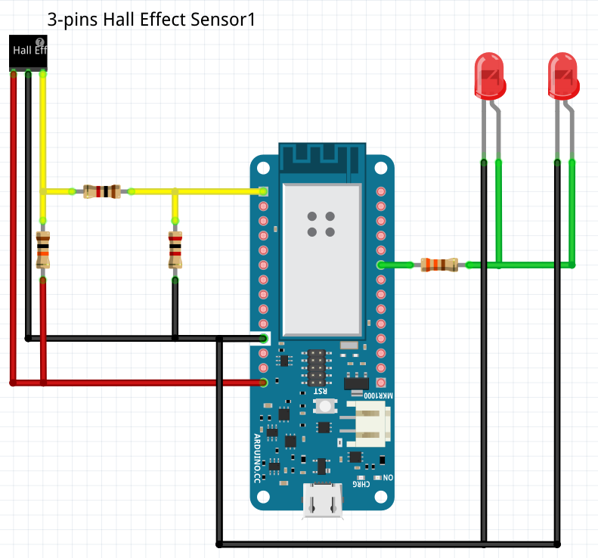
\includegraphics[
    width=0.5\linewidth,
    ]{imgs/hardware_car_iteration1.png}
    \caption{Erstes Konzept des Schaltplans für die Fahrzeuge}
    \label{fig-hardware-car-iteration1}
\end{center}
\end{figure}
\noindent
Mit einem $1k\ \Omega$ und $2k\ \Omega$ Widerstand können Spannungen von $5V$ 
auf $3.3V$ runter gesetzt werden. Neben diesen Widerständen soll ein 
$10k\ \Omega$ Pull-Up Widerstand verwendet werden, welcher den verwendeten Pin 
des Arduinos auf $HIGH$ zieht, solange kein Magnet erkannt ist. Das verwendete 
Diagramm ist in Abbildung \ref{fig-hardware-car-iteration1} dargestellt. 
Hierbei werden zwei LEDs hinzugefügt, welche später als Scheinwerfer in 
dem Fahrzeug verwendet werden. Beim Testen fällt auf, dass die Kombination aus 
Pegelwandler und dem Pull-Up Widerstand nicht funktioniert und kein Auslesen 
von Sensorwerten möglich ist.
\end{document}